\documentclass[11pt,a4paper]{article}

% ---- Packages ----------------------------------------------------------
\usepackage[utf8]{inputenc}
\usepackage[T1]{fontenc}
\usepackage{lmodern}
\usepackage[margin=0.9in]{geometry}
\usepackage{microtype}
\usepackage{amsmath}
\usepackage{amssymb}
\usepackage{titlesec}
\usepackage{enumitem}
\usepackage{booktabs}
\usepackage{array}
\usepackage{tabularx}
\usepackage{xcolor}
\usepackage{graphicx}
\usepackage{fancyhdr}
\usepackage{tikz}
\usetikzlibrary{positioning, arrows.meta, shapes.geometric, fit, calc, backgrounds, decorations.pathreplacing}
\usepackage[hidelinks,colorlinks=true,linkcolor=black,citecolor=teal,urlcolor=teal]{hyperref}
\usepackage{parskip}
\usepackage{float}

% ---- Color palette -----------------------------------------------------
\definecolor{accent}{HTML}{0F766E}
\definecolor{accentlight}{HTML}{CCFBF1}
\definecolor{warm}{HTML}{B45309}
\definecolor{warmlight}{HTML}{FEF3C7}
\definecolor{cool}{HTML}{1E3A8A}
\definecolor{coollight}{HTML}{DBEAFE}
\definecolor{neutral}{HTML}{475569}
\definecolor{neutrallight}{HTML}{F1F5F9}

% ---- TikZ styles -------------------------------------------------------
\tikzset{
  data/.style    = {rectangle, rounded corners=3pt, draw=neutral, thick,
                    fill=neutrallight, minimum width=2.4cm, minimum height=0.85cm,
                    align=center, font=\small},
  proc/.style    = {rectangle, rounded corners=3pt, draw=cool, thick,
                    fill=coollight, minimum width=2.4cm, minimum height=0.85cm,
                    align=center, font=\small},
  model/.style   = {rectangle, rounded corners=3pt, draw=accent, very thick,
                    fill=accentlight, minimum width=3.0cm, minimum height=1.0cm,
                    align=center, font=\small},
  artifact/.style= {rectangle, rounded corners=3pt, draw=warm, thick,
                    fill=warmlight, minimum width=2.4cm, minimum height=0.85cm,
                    align=center, font=\small},
  device/.style  = {rectangle, rounded corners=3pt, draw=neutral, thick,
                    fill=neutrallight, minimum width=2.0cm, minimum height=0.7cm,
                    align=center, font=\small},
  alert/.style   = {rectangle, rounded corners=3pt, draw=red!60!black, thick,
                    fill=red!8, minimum width=2.4cm, minimum height=0.85cm,
                    align=center, font=\small},
  pkt/.style     = {rectangle, draw=cool!70, thick, fill=coollight,
                    minimum width=0.55cm, minimum height=0.55cm,
                    inner sep=1pt, font=\tiny},
  feat/.style    = {circle, draw=accent!70, thick, fill=accentlight,
                    inner sep=1pt, minimum size=0.45cm, font=\tiny},
  fuse/.style    = {diamond, draw=warm, thick, fill=warmlight,
                    aspect=2, inner sep=1pt, align=center, font=\small},
  arr/.style     = {-{Latex[length=2mm,width=1.6mm]}, thick, draw=neutral!80},
  darr/.style    = {-{Latex[length=2mm,width=1.6mm]}, thick, draw=neutral!80, dashed},
}

% ---- Header / Footer ---------------------------------------------------
\pagestyle{fancy}
\fancyhf{}
\fancyhead[L]{\small Mamba IoT Anomaly Detection}
\fancyhead[R]{\small Madhav Dogra}
\fancyfoot[C]{\thepage}
\renewcommand{\headrulewidth}{0.4pt}

% ---- Section formatting (tighter) --------------------------------------
\titleformat{\section}{\normalfont\large\bfseries\color{cool}}{\thesection}{0.6em}{}
\titlespacing*{\section}{0pt}{6pt}{2pt}

\setlength{\parskip}{4pt}

% =======================================================================
\begin{document}

\begin{center}
{\Large\bfseries Flow-Pattern Anomaly Detection at the IoT Gateway} \\[2pt]
{\small Madhav Dogra}
\end{center}

\vspace{-4pt}

% =======================================================================
\section{Aim}
Detect bad traffic from \textbf{smart-home IoT devices} (cameras, sensors, smart bulbs, voice assistants, thermostats, doorbells, smart plugs) at the home gateway. Catch known attacks and zero-days. Works on encrypted traffic. Runs under 10\,ms on Raspberry-Pi-class hardware.

\section{Why the gateway}
Smart-home IoT endpoints can't run an agent --- weak firmware, no patches, no compute. Gateway is the choke point. Every flow passes through. Only place where modern compute can sit.

% ---- Figure 1: Deployment context --------------------------------------
\begin{figure}[H]
\centering
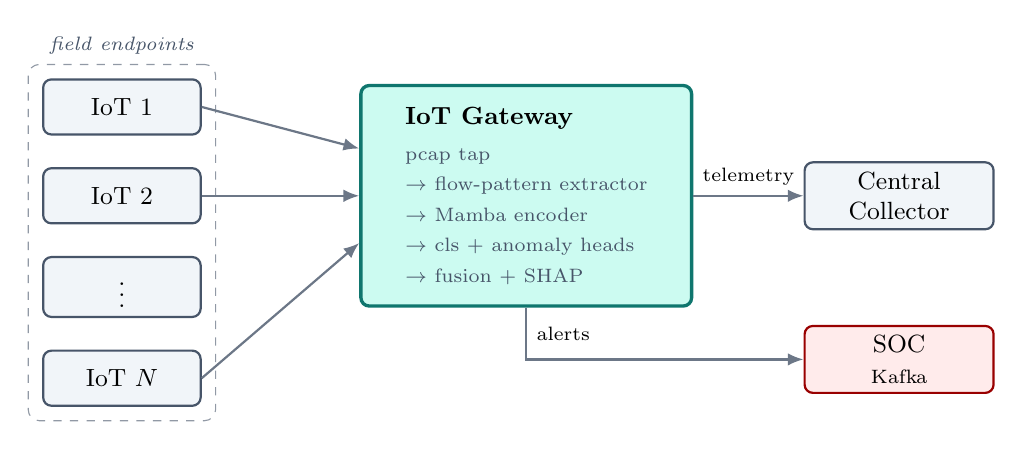
\begin{tikzpicture}[node distance=0.4cm and 1.2cm]

  \node[device]                  (d1) {IoT 1};
  \node[device, below=of d1]     (d2) {IoT 2};
  \node[device, below=of d2]     (d3) {\vdots};
  \node[device, below=of d3]     (dn) {IoT $N$};

  \node[draw=neutral!60, dashed, rounded corners, fit=(d1)(dn), inner sep=5pt,
        label={[font=\scriptsize\itshape, neutral]above:field endpoints}] (grp) {};

  \node[model, right=2.0cm of d2, minimum width=4.2cm, minimum height=2.8cm,
        align=left] (gw) {\textbf{IoT Gateway}\\[2pt]
        \scriptsize\textcolor{neutral}{pcap tap}\\
        \scriptsize\textcolor{neutral}{$\to$ flow-pattern extractor}\\
        \scriptsize\textcolor{neutral}{$\to$ Mamba encoder}\\
        \scriptsize\textcolor{neutral}{$\to$ cls + anomaly heads}\\
        \scriptsize\textcolor{neutral}{$\to$ fusion + SHAP}};

  \node[data, right=1.4cm of gw, minimum width=2.4cm] (cc) {Central \\ Collector};
  \node[alert, below=1.2cm of cc, minimum width=2.4cm] (soc) {SOC \\ \scriptsize Kafka};

  \draw[arr] (d1.east) -- ([yshift=0.6cm]gw.west);
  \draw[arr] (d2.east) -- (gw.west);
  \draw[arr] (dn.east) -- ([yshift=-0.6cm]gw.west);
  \draw[arr] (gw.east) -- node[above, font=\scriptsize]{telemetry} (cc.west);
  \draw[arr] (gw.south) |- node[pos=0.25, right, font=\scriptsize]{alerts} (soc.west);

\end{tikzpicture}
\caption*{\small\textit{Detector lives inside the gateway. Telemetry passes through untouched; alerts go out-of-band to the SOC.}}
\end{figure}

% =======================================================================
\section{The input: flow patterns, not aggregates}
Standard IDS reduces each flow to $\sim$80 summary stats. Order is gone. Attack signatures live in order. Instead --- keep the first $K\!\approx\!32$ packets of the flow as a sequence. Each packet $p_t$ = size, direction, IAT, flags, header bytes. Payload-free, so encrypted traffic still works.

% ---- Figure 2: Representation contrast (vertical) ----------------------
\begin{figure}[H]
\centering
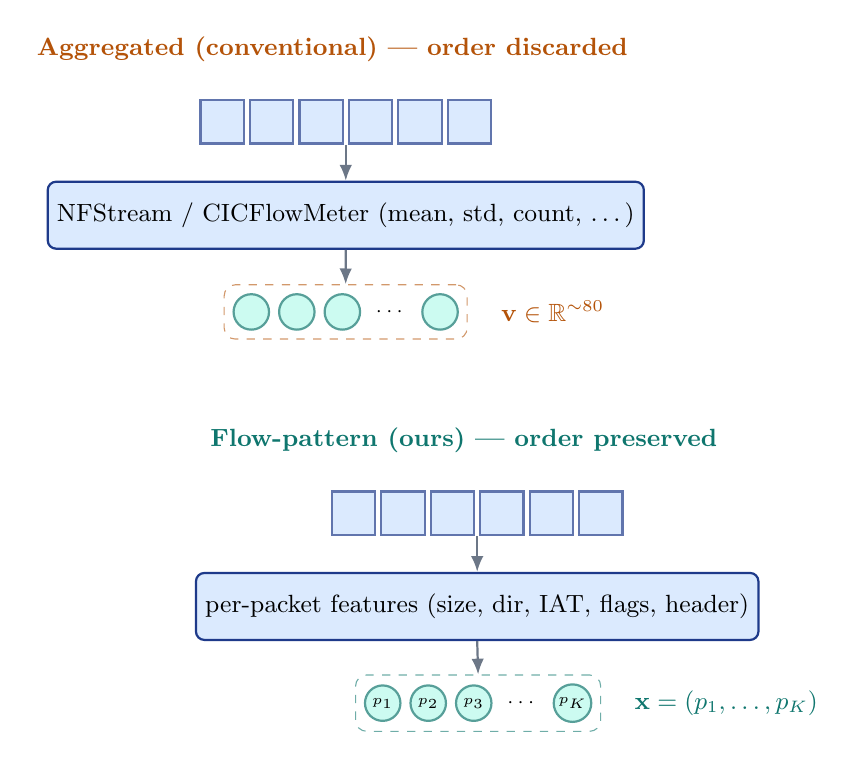
\begin{tikzpicture}[node distance=0.4cm and 0.8cm]

  % TOP: Aggregated
  \node[font=\bfseries\small, color=warm] (lhd) {Aggregated (conventional) --- order discarded};

  \node[pkt, below=0.35cm of lhd, xshift=-1.4cm] (lp1) {};
  \node[pkt, right=0.05cm of lp1] (lp2) {};
  \node[pkt, right=0.05cm of lp2] (lp3) {};
  \node[pkt, right=0.05cm of lp3] (lp4) {};
  \node[pkt, right=0.05cm of lp4] (lp5) {};
  \node[pkt, right=0.05cm of lp5] (lp6) {};
  \node[fit=(lp1)(lp6), inner sep=0pt] (lpkts) {};

  \node[proc, below=0.45cm of lpkts, minimum width=5.2cm] (lagg)
       {\small NFStream / CICFlowMeter (mean, std, count, \ldots)};

  \node[feat, below=0.55cm of lagg, xshift=-1.2cm] (lf1) {};
  \node[feat, right=0.1cm of lf1] (lf2) {};
  \node[feat, right=0.1cm of lf2] (lf3) {};
  \node[right=0.06cm of lf3, font=\scriptsize] (ldots) {$\cdots$};
  \node[feat, right=0.06cm of ldots] (lf4) {};

  \node[draw=warm!60, dashed, rounded corners, fit=(lf1)(lf4), inner sep=3pt] (lvec) {};
  \node[right=0.3cm of lvec, font=\small, color=warm] {$\mathbf{v}\in\mathbb{R}^{\sim 80}$};

  \draw[arr] (lpkts.south) -- (lagg.north);
  \draw[arr] (lagg.south) -- (lvec.north);

  % BOTTOM: Flow-pattern
  \node[font=\bfseries\small, color=accent, below=1.0cm of lvec, xshift=1.5cm] (rhd)
       {Flow-pattern (ours) --- order preserved};

  \node[pkt, below=0.35cm of rhd, xshift=-1.4cm] (rp1) {};
  \node[pkt, right=0.05cm of rp1] (rp2) {};
  \node[pkt, right=0.05cm of rp2] (rp3) {};
  \node[pkt, right=0.05cm of rp3] (rp4) {};
  \node[pkt, right=0.05cm of rp4] (rp5) {};
  \node[pkt, right=0.05cm of rp5] (rp6) {};
  \node[fit=(rp1)(rp6), inner sep=0pt] (rpkts) {};

  \node[proc, below=0.45cm of rpkts, minimum width=5.2cm] (ragg)
       {\small per-packet features (size, dir, IAT, flags, header)};

  \node[feat, below=0.55cm of ragg, xshift=-1.2cm] (rf1) {$p_1$};
  \node[feat, right=0.1cm of rf1] (rf2) {$p_2$};
  \node[feat, right=0.1cm of rf2] (rf3) {$p_3$};
  \node[right=0.06cm of rf3, font=\scriptsize] (rdots) {$\cdots$};
  \node[feat, right=0.06cm of rdots] (rf4) {$p_K$};

  \node[draw=accent!60, dashed, rounded corners, fit=(rf1)(rf4), inner sep=3pt] (rvec) {};
  \node[right=0.3cm of rvec, font=\small, color=accent] {$\mathbf{x}=(p_1,\ldots,p_K)$};

  \draw[arr] (rpkts.south) -- (ragg.north);
  \draw[arr] (ragg.south) -- (rvec.north);

\end{tikzpicture}
\caption*{\small\textit{Top: collapse to summary stats, lose temporal structure. Bottom: keep the packets in order. Sequence model does the aggregation.}}
\end{figure}

% =======================================================================
\section{The model}
\begin{itemize}[leftmargin=*, itemsep=1pt, topsep=2pt]
  \item One \textbf{Mamba encoder}. Pre-trained self-supervised on benign-only flows. Produces an embedding $\mathbf{z}$.
  \item Two heads share it. \textbf{Classifier} for 7 known classes reads $\mathbf{z}$ directly. \textbf{Anomaly head} (deep SVDD) reads a learned \textbf{projection} $\mathbf{z}_\text{ano}$ in a lower-dimensional space --- one-class methods are sensitive to the curse of dimensionality, so we project down first.
  \item Either head fires $\Rightarrow$ alert. SHAP attributions over the sequence. Sent to SOC over Kafka.
  \item Why Mamba and not a transformer? ET-BERT works but is $\sim$100M params --- doesn't fit a gateway. NetMamba shows you get ET-BERT-class accuracy on a Mamba backbone at a fraction of the cost. Linear-time inference in $K$.
\end{itemize}

% ---- Figure 3: Inference pipeline --------------------------------------
\begin{figure}[H]
\centering
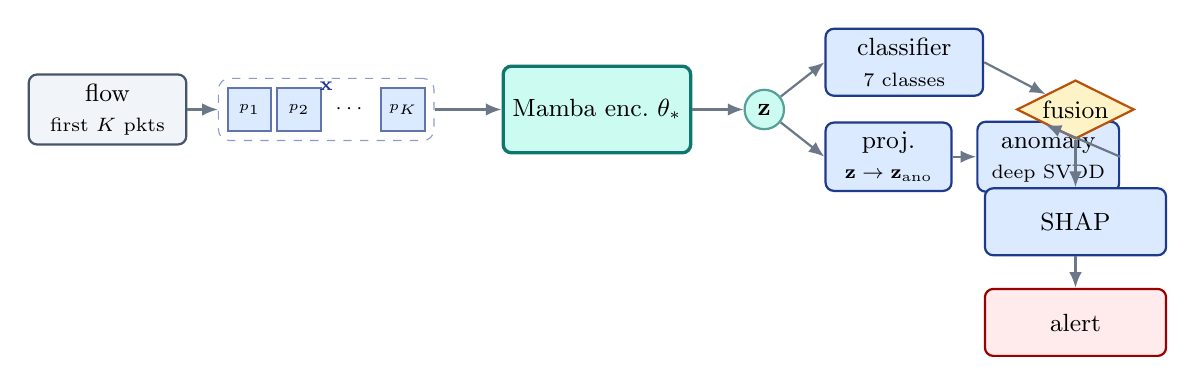
\begin{tikzpicture}[node distance=0.5cm and 0.6cm]

  \node[data, minimum width=2.0cm] (raw) {flow \\ \scriptsize first $K$ pkts};

  \node[pkt, right=0.5cm of raw] (p1) {$p_1$};
  \node[pkt, right=0.05cm of p1] (p2) {$p_2$};
  \node[right=0.05cm of p2, font=\scriptsize] (pdots) {$\cdots$};
  \node[pkt, right=0.05cm of pdots] (pk) {$p_K$};
  \node[draw=cool!50, dashed, rounded corners, fit=(p1)(pk), inner sep=3pt,
        label={[font=\scriptsize, below=-2pt, cool]:$\mathbf{x}$}] (seq) {};

  \node[model, right=0.85cm of seq, minimum width=2.3cm, minimum height=1.1cm] (enc)
       {Mamba enc.\ $\theta_*$};

  \node[feat, right=0.65cm of enc, minimum size=0.5cm, font=\small] (z) {$\mathbf{z}$};

  \node[proc, right=0.5cm of z, yshift=0.6cm, minimum width=2.0cm] (cls)
       {classifier \\ \scriptsize 7 classes};
  \node[proc, right=0.5cm of z, yshift=-0.6cm, minimum width=1.6cm] (proj)
       {proj. \\ \scriptsize $\mathbf{z}\to\mathbf{z}_\text{ano}$};
  \node[proc, right=0.3cm of proj, minimum width=1.8cm] (ano)
       {anomaly \\ \scriptsize deep SVDD};

  \node[fuse, right=0.4cm of cls, yshift=-0.6cm] (fuse) {fusion};

  \node[proc, below=0.6cm of fuse, minimum width=2.3cm] (shap)
       {SHAP};
  \node[alert, below=0.4cm of shap, minimum width=2.3cm] (out) {alert};

  \draw[arr] (raw) -- (seq);
  \draw[arr] (seq) -- (enc);
  \draw[arr] (enc) -- (z);
  \draw[arr] (z) -- (cls.west);
  \draw[arr] (z) -- (proj.west);
  \draw[arr] (proj) -- (ano);
  \draw[arr] (cls.east) -- (fuse.north west);
  \draw[arr] (ano.east) -- (fuse.south west);
  \draw[arr] (fuse.south) -- (shap.north);
  \draw[arr] (shap.south) -- (out.north);

\end{tikzpicture}
\caption*{\small\textit{One encoder, two heads. Anomaly head sees a lower-dim projection of $\mathbf{z}$. Either fires $\Rightarrow$ alert. SHAP explains it.}}
\end{figure}

% =======================================================================
\section{Training: three stages}
\begin{enumerate}[leftmargin=*, itemsep=1pt, topsep=2pt]
  \item \textbf{Pre-train.} Mamba on unlabelled benign flows. Masked-pattern objective. No attack labels.
  \item \textbf{Fine-tune.} Init from pre-trained weights. Joint train encoder + classifier on labelled CICIoT2023. Focal loss for imbalance.
  \item \textbf{Anomaly head.} Freeze encoder. Embed a held-out benign set. Fit one-class scorer on those embeddings. Threshold at 99th percentile (1\% FPR target).
\end{enumerate}

Zero-day test: leave-one-class-out --- hide attack classes from the supervised head and check the anomaly head catches them.

% ---- Figure 4: Training pipeline ---------------------------------------
\begin{figure}[H]
\centering
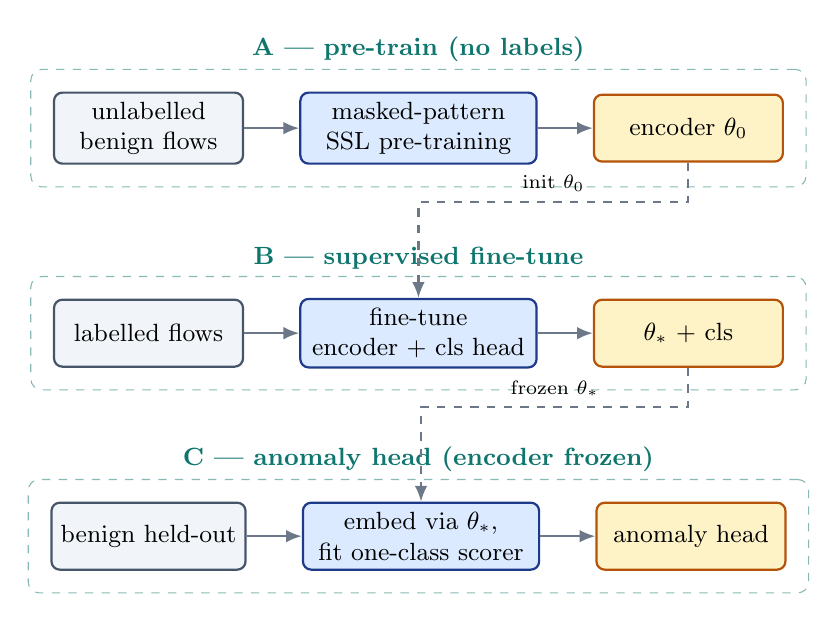
\begin{tikzpicture}[node distance=0.5cm and 0.7cm]

  % Stage A
  \node[data, minimum width=2.4cm] (a1) {unlabelled \\ benign flows};
  \node[proc, right=of a1, minimum width=3.0cm] (a2)
       {masked-pattern \\ SSL pre-training};
  \node[artifact, right=of a2, minimum width=2.4cm] (a3) {encoder $\theta_0$};
  \node[draw=accent!50, dashed, rounded corners, fit=(a1)(a3), inner sep=8pt,
        label={[font=\small\bfseries, accent, above=-1pt]:A --- pre-train (no labels)}] (sA) {};
  \draw[arr] (a1) -- (a2);
  \draw[arr] (a2) -- (a3);

  % Stage B
  \node[data, minimum width=2.4cm, below=1.7cm of a1] (b1)
       {labelled flows};
  \node[proc, right=of b1, minimum width=3.0cm] (b2)
       {fine-tune \\ encoder + cls head};
  \node[artifact, right=of b2, minimum width=2.4cm] (b3) {$\theta_*$ + cls};
  \node[draw=accent!50, dashed, rounded corners, fit=(b1)(b3), inner sep=8pt,
        label={[font=\small\bfseries, accent, above=-1pt]:B --- supervised fine-tune}] (sB) {};
  \draw[arr] (b1) -- (b2);
  \draw[arr] (b2) -- (b3);
  \draw[darr] (a3.south) -- ++(0,-0.5) -| node[pos=0.25, above, font=\scriptsize]{init $\theta_0$} (b2.north);

  % Stage C
  \node[data, minimum width=2.4cm, below=1.7cm of b1] (c1) {benign held-out};
  \node[proc, right=of c1, minimum width=3.0cm] (c2)
       {embed via $\theta_*$, \\ fit one-class scorer};
  \node[artifact, right=of c2, minimum width=2.4cm] (c3) {anomaly head};
  \node[draw=accent!50, dashed, rounded corners, fit=(c1)(c3), inner sep=8pt,
        label={[font=\small\bfseries, accent, above=-1pt]:C --- anomaly head (encoder frozen)}] (sC) {};
  \draw[arr] (c1) -- (c2);
  \draw[arr] (c2) -- (c3);
  \draw[darr] (b3.south) -- ++(0,-0.5) -| node[pos=0.25, above, font=\scriptsize]{frozen $\theta_*$} (c2.north);

\end{tikzpicture}
\caption*{\small\textit{Three stages. Encoder built without labels, specialised with labels, then anomaly head added on top.}}
\end{figure}

% =======================================================================
\section{Two modes --- default + strong (admin-switched)}
Gateway runs in one of two configurations. Admin picks. Not a per-flow decision.
\begin{itemize}[leftmargin=*, itemsep=1pt, topsep=2pt]
  \item \textbf{Default} (always on, low power). Small $K$, smallest Mamba, anomaly head only, no SHAP. Target $<$2\,ms / flow. Continuous operation on Raspberry-Pi-class hardware.
  \item \textbf{Strong} (admin-switched, full pipeline). $K\!=\!32$, full encoder, both heads (with projection on the anomaly side), SHAP on every alert. Target $<$10\,ms / flow. Switched on for elevated threat, incident response, or high-value windows.
\end{itemize}
Same model artifacts in both modes --- what differs is which components are engaged and at what size.

% =======================================================================
\section{Progressive learning --- new attacks}
When a new attack type appears:
\begin{enumerate}[leftmargin=*, itemsep=1pt, topsep=2pt]
  \item \textbf{Day-zero}: anomaly head flags it (it just looks unlike normal).
  \item \textbf{Label}: SOC confirms and labels a sample.
  \item \textbf{Update head only}: add a class to the classifier softmax, fine-tune just the head on the new data with a replay buffer. \textbf{Encoder stays frozen.} Takes minutes, not days.
  \item \textbf{Recalibrate threshold} on a fresh benign set if needed.
\end{enumerate}
Full encoder retraining is only needed if \emph{benign} traffic itself shifts. ``What's normal'' (encoder, expensive) and ``what's malicious'' (heads, cheap) are decoupled --- that's the whole point of the shared-encoder design.

% =======================================================================
\section{Evaluation}
\begin{itemize}[leftmargin=*, itemsep=1pt, topsep=2pt]
  \item \textbf{Datasets.} CICIoT2023 (primary). TON\_IoT (cross-dataset). IoT-23 (malware).
  \item \textbf{Baselines.} ET-BERT (upper bound, gateway-infeasible). CNN-BiLSTM on aggregated stats (representation control). \textbf{XGBoost} (classical-floor challenge --- ``do we need deep learning at all?''; the deep model earns its complexity only on zero-day, cross-dataset, and adversarial metrics, where XGBoost can't compete). Isolation Forest (classical unsupervised floor).
  \item \textbf{Metrics.} Per-class P/R/F1. PR-AUC. p50/p95/p99 latency. Model size after int8 quantisation.
  \item \textbf{Adversarial.} FGSM on the sequence. Plot detection rate vs $\varepsilon$. Both heads.
  \item \textbf{Edge benchmark.} Raspberry-Pi-class hardware. Target $<$10\,ms p95 per flow.
\end{itemize}

% =======================================================================
\section{Deliverables}
Code repo. Pre-trained encoder checkpoint. Benchmark table (5 baselines $\times$ 3 datasets). FGSM curves. Edge-hardware latency profile. Written report.

% =======================================================================
\section{Risks --- and what I do about them}
\begin{itemize}[leftmargin=*, itemsep=1pt, topsep=2pt]
  \item Pre-training compute blows budget $\to$ warm-start from a public Mamba checkpoint.
  \item Class imbalance hides minority-class failure $\to$ focal loss + per-class metrics.
  \item Cross-dataset accuracy drop $\to$ measure honestly, don't hide.
  \item Edge memory overrun $\to$ int8 quantise; fall back to smaller config; reduce $K$.
  \item Byte-level adversarial sensitivity $\to$ FGSM study quantifies it; SHAP fingerprint as secondary defence.
\end{itemize}

% =======================================================================
\section{Stretch goals}
\begin{itemize}[leftmargin=*, itemsep=1pt, topsep=2pt]
  \item Swap Mamba $\to$ Mamba-2 (SSD) if latency headroom allows.
  \item Add E-GraphSAGE branch over a per-window device graph.
  \item Federated pre-training across multiple sites.
\end{itemize}

% =======================================================================
\section{Key references}
\footnotesize
ET-BERT \href{https://arxiv.org/abs/2202.06335}{(arxiv 2202.06335)} \textbullet\
NetMamba \href{https://arxiv.org/abs/2405.11449}{(2405.11449)} \textbullet\
Mamba \href{https://arxiv.org/abs/2312.00752}{(2312.00752)} \textbullet\
Mamba-2 / SSD \href{https://arxiv.org/abs/2405.21060}{(2405.21060)} \textbullet\
S4D \href{https://arxiv.org/abs/2206.11893}{(2206.11893)} \textbullet\
CICIoT2023 \href{https://www.mdpi.com/1424-8220/23/13/5941}{(MDPI Sensors)} \textbullet\
ET-SSL \href{https://www.nature.com/articles/s41598-025-08568-0}{(Nature Sci.Rep.)} \textbullet\
E-GraphSAGE \href{https://arxiv.org/abs/2103.16329}{(2103.16329)}.

\end{document}
